\newpage
\section{Linear material models}
The set of linear models in Voigt notation can be expressed by the following
equation,
\begin{eqnarray}
\beps   &=& \bbD_{\bfE,T}\bsig + \bfd_{\bsig,T}   \bfE + \balpha_{\bsig,\bfE}\Delta T \\
\bfD    &=& \bfd_{\bfE,T}\bsig + \bkappa_{\bsig,T}\bfE + \bfp_{\bsig}\Delta T \\
\Delta S&=& \balpha_{\bfE,T}   + \bfp_{\bsig,T}   \bfE + \frac{C_{\bsig,\bfE}}{T}\Delta T
\end{eqnarray}
or in matrix notation,
\begin{eqnarray}
\left[
\begin{array}{c}
\beps  \\
\bfD   \\
\Delta S
\end{array}
\right]
&=&
\left[
\begin{array}{ccc}
\bbD_{\bfE,T}       & \bfd_{\bsig,T}     & \balpha_{\bsig,\bfE}    \\
\bfd_{\bfE,T}^T    & \bkappa_{\bsig,T}   & \bfp_{\bsig,\bfE}       \\
\balpha_{\bfE,T}^T & \bfp_{\bsig,T}^T    & \frac{C_{\bsig,\bfE}}{T}
\end{array}
\right]
\left[
\begin{array}{c}
\bsig \\
\bfE \\
\Delta T
\end{array}
\right]
\end{eqnarray}
Here,
$\beps$ denotes the linearized strain tensor, $\bsig$ the stress tensor, 
$\bfD$  the electric displacement, $\bfE$ the electric field,
$\Delta S$ the change in entropy, and $\Delta T$ the change in temperature.
The material dependent coeficients are denoted by,
$\bfs$ the compliance tensor, $\bfd$ the piezoelectric strain coeficient,
$\balpha$ the linear thermal expansion coeficient, 
$\bkappa$ the dielectric coeficient, $\bfp$ the pyroelectric coeficient,
$C$ the heat capacity, and $T$ is the reference temperature. The subscripts 
denote the fields which are taken
as constant in evaluating the coeficients.
We assume these coficients are represented in Voigt notation shown 
in Table \ref{table:VoigtNotation}
\begin{table}[htbp]
\caption{Voigt notation}
\label{table:VoigtNotation}
\begin{center}
\begin{tabular}{|c|cccccc|}
\hline
Voigt    &  1    &  2    &  3    &  4    &   5    &  6   \\
\hline
$(i,j)$  & (1,1) & (2,2) & (3,3) & (1,2) &  (2,3) & (3,1)\\
\hline
\end{tabular}
\end{center}
\end{table}
Additionally, the strain tensor in vector form is represented by,
\begin{eqnarray}
\beps &=& \left[ \beps_{11}, \beps_{22}, \beps_{33}, 2\beps_{12}, 2\beps_{23}, 2\beps_{31} \right]^T
\end{eqnarray}

Depending on the fields that are coupled, certain portions of the relation
above are extracted. Often, instead of the compliance $\bbD$, the inverse 
value representing the stiffness $\bbC=\bbD^{-1}$ is used. The number of 
material constants required to represent the material differ depending on
the geometry. 
These are summarized in Table \ref{table:CrystalDependentMaterialConstants}.

\begin{table}[htbp]
\centering
\caption{Material constants for different crystals}
\label{table:CrystalDependentMaterialConstants}
\begin{tabular}{|c||c|c|c|c|c|}
\hline
Crystal & Elastic($\bbC$) & Piezo($\bfd$) & Thermal($\balpha$) & Dielectric($\bkappa$) & Pyro($\bfp$) \\
\hhline{|=||=|=|=|=|=|}
Isotropic & $\bbC_{12}$,$\bbC_{44}$ & (-)   & $\balpha_T$     & $\bkappa$           & (-)          \\
\hline
Cubic     & $\bbC_{11}$,$\bbC_{12}$,$\bbC{44}$ & (-)& $\balpha_T$         & $\bkappa$             & (-)          \\
\hline
Hexagonal & $\bbC_{11}$,$\bbC_{12}$,$\bbC_{13}$,$\bbC_{33}$,$\bbC_{55}$ & $\bfd_{16}$,$\bfd_{31}$,$\bfd_{33}$
                                          & $\balpha_{T1}$,$\balpha_{T2}$ 
                                                               & $\bkappa_1$,$\bkappa_2$& (-)         \\
\hline
\end{tabular}
\end{table}

\clearpage
\subsection{Elasticity }
For elasticity, only the terms relatin stress and strain are 
extracted. The compliance tensor is inverted to obtain stress in
terms of strain as,
\begin{eqnarray}
\bsig = \bbC\beps \\
\bbC  = \bbD^{-1}
\end{eqnarray} 
The number of elastic constants that must be specified differ 
depending on the symmetry of the crystal.

\subsubsection{Isotropic material}
\begin{flushleft}
  \textbf{Required parameters in \ttt{mtype}:}
  [\ttt{E} and \ttt{nu}] or [\ttt{lambda} and \ttt{mu}]
\end{flushleft}

Two numbers define the elastic properties of an isotropic material.
In matrix form the stiffness is,
\begin{eqnarray}
\bbC_\text{isotropic} &=&
\left[
\begin{array}{cccccc}
\bbC_{12}+2\bbC_{44}  & \bbC_{12}  &  \bbC_{12}  &   0   &   0    &  0    \\
\bbC_{12}  & \bbC_{12}+2\bbC_{44} &  \bbC_{12}  &   0   &   0    &  0    \\
\bbC_{12}  & \bbC_{12}  &  \bbC_{12}+2\bbC_{44} &   0   &   0    &  0    \\
    0   &     0   &      0   & \bbC_{44} & 0 & 0 \\
    0   &     0   &      0   &   0   & \bbC_{44} &  0    \\
    0   &     0   &      0   &   0   &   0    & \bbC_{44}
\end{array}
\right] 
\end{eqnarray}
The values $\bbC_{12}$ and $\bbC_{44r}$ correspond to the Lame
constants $\lambda$ and $\mu$ and are related to the Youngs modulus
$E$ and Poisson ratio $\nu$ by,
\begin{eqnarray}
\bbC_{12} &=& \lambda = \frac{\nu E}{(1-2\nu)(1+\nu)} \\
\bbC_{44} &=& \mu     = \frac{E}{2(1+\nu)}
\end{eqnarray}
We can express the material tensors in a coordinate free notation
where given crystal
axes orientation $[\bfa,\bfb,\bfc]$, the elasticity tensor can be
expressed as,
\begin{eqnarray}
\bbC_{cubic} &=&  \bbC_{12}\rkTwoI\otimes\rkTwoI
                +2\bbC_{44}\rkFourIsym  \nonumber
\end{eqnarray}

\subsubsection{Cubic material}
\begin{flushleft}
  \textbf{Required parameters in \ttt{mtype}:}
  [\ttt{alpha}, \ttt{lambda}, and \ttt{mu}]
\end{flushleft}

Two numbers define the elastic properties of an isotropic material.
In matrix form the stiffness is,
\begin{eqnarray}
\bbC_\text{cubic} &=&
\left[
\begin{array}{cccccc}
\bbC_{11}  & \bbC_{12}  &  \bbC_{12}  &   0   &   0    &  0    \\
\bbC_{12}  & \bbC_{11}  &  \bbC_{12}  &   0   &   0    &  0    \\
\bbC_{12}  & \bbC_{12}  &  \bbC_{11}  &   0   &   0    &  0    \\
    0   &     0   &      0   & \bbC_{44} & 0 & 0 \\
    0   &     0   &      0   &   0   & \bbC_{44} &  0    \\
    0   &     0   &      0   &   0   &   0    & \bbC_{44}
\end{array}
\right]
\end{eqnarray}
The cubic coefficients are related to the usual expression for cubic
materials $\lambda, \mu, \alpha$ by the relations,
\begin{eqnarray}
\bbC_{11} &=& \alpha  \nonumber \\
\bbC_{12} &=& \lambda \nonumber \\
\bbC_{44} &=& \mu     \nonumber
\end{eqnarray}

We can express the material tensors in a coordinate free notation
where given
the cubic coeffecients $c_{11},c_{12},c_{c44}$ and crystal
axes orientation $[\bfa,\bfb,\bfc]$, the elasticity tensor can be
expressed as,
\begin{eqnarray}
\bbC_{cubic} &=&  c_{12}\rkTwoI\otimes\rkTwoI
                +2c_{44}\rkFourIsym
                + \left( c_{11}-c_{12}-2c_{44} \right)
                  \left(   \bfa \otimes \bfa \otimes \bfa \otimes \bfa
                         + \bfb \otimes \bfb \otimes \bfb \otimes \bfb
                         + \bfc \otimes \bfc \otimes \bfc \otimes \bfc \right)
                                                  \nonumber
\end{eqnarray}

\subsubsection{Hexagonal material}
\begin{flushleft}
  \textbf{Required parameters in \ttt{mtype}:}
  [\ttt{c11}, \ttt{c12}, \ttt{c13}, \ttt{c33}, and \ttt{c55}]
\end{flushleft}

The crystal has an in plane hexagonal structure giving
it an isotropic property in plane. The material begin piezoelectric
has no center of symmetry(inversion center). A hexagonal
crystal has the following structure for the elasticity tensor
$bbC_{hex}$, piezoelectric strain coefficients $\bfd_{hex}$ and
dielectric constants $\bkappa_{d\bsig}$ in Voigt notation.
The 1,2 axes are assumed to be in the isotropic crystal
plane with the 3 axis perpendicular to this plane.


\begin{eqnarray}
\bbC_{hex} &=&
\left[
\begin{array}{cccccc}
c_{11}  & c_{12}  &  c_{13}  &   0   &   0    &  0    \\
c_{12}  & c_{11}  &  c_{13}  &   0   &   0    &  0    \\
c_{13}  & c_{13}  &  c_{33}  &   0   &   0    &  0    \\
    0   &     0   &      0   & \frac{c_{11}-c_{12}}{2} & 0 & 0 \\
    0   &     0   &      0   &   0   & c_{55} &  0    \\
    0   &     0   &      0   &   0   &   0    & c_{55}
\end{array}
\right] 
\end{eqnarray}

In a hexagonal material, given the stiffness coefficients,
$c_{11},c_{12},c_{13},c_{33},c_{55}$, the elasticity tensor can
be expressed as,
\begin{eqnarray}
\bbC_{hex}  &=&                   c_{12}        \rkTwoI\otimes\rkTwoI
                + \left( c_{11} - c_{12} \right)\rkFourIsym
                                                    \nonumber\\
            & & + \left( c_{33} - c_{11} \right)
                  \left(   \bfc \otimes \bfc \otimes \bfc \otimes \bfc \right)
                                                    \nonumber\\
            & & + \left( c_{13} - c_{12} \right)
                  \left(   \bfa \otimes \bfa \otimes \bfc \otimes \bfc
                         + \bfc \otimes \bfc \otimes \bfa \otimes \bfa
                         + \bfb \otimes \bfb \otimes \bfc \otimes \bfc
                         + \bfc \otimes \bfc \otimes \bfb \otimes \bfb \right)
                                                     \nonumber\\
            & & + \left( c_{55} - \frac{c_{11}-c_{12}}{2} \right)
                  \left(   \bfb \otimes \bfc \otimes \bfb \otimes \bfc
                         + \bfb \otimes \bfc \otimes \bfc \otimes \bfb
                         + \bfc \otimes \bfb \otimes \bfb \otimes \bfc
                         + \bfc \otimes \bfb \otimes \bfc \otimes \bfb \right)
                                                     \nonumber\\
            & & + \left( c_{55} - \frac{c_{11}-c_{12}}{2} \right)
                  \left(   \bfc \otimes \bfa \otimes \bfc \otimes \bfa
                         + \bfc \otimes \bfa \otimes \bfa \otimes \bfc
                         + \bfa \otimes \bfc \otimes \bfc \otimes \bfa
                         + \bfa \otimes \bfc \otimes \bfa \otimes \bfc \right)
                                                     \nonumber
\end{eqnarray}


\clearpage
\subsection{Thermoelasticity }
For thermoelasticity, the terms relating stress,strain,entropy and temperature are
extracted. The compliance tensor is inverted to obtain stress in
terms of strain as,
\begin{eqnarray}
\left[
\begin{array}{c}
\bsig \\
\Delta S 
\end{array}
\right]
&=&
\left[
\begin{array}{cc}
\bbC & -\bbC\balpha \\
\balpha^T\bbC & \frac{C}{T}-\balpha^T\bbC\balpha
\end{array}
\right]
\left[
\begin{array}{c}
\beps \\
\Delta T
\end{array}
\right]
\end{eqnarray}
Additional to this, a constitutive equation must be given
for the heat flux $\bfq$. Standard linear Fourier model is assumed.
\begin{eqnarray}
\bfq = \bkappa_T\bfnabla T
\end{eqnarray}
where, $\bkappa_T$ is the conductivity tensor.

\subsubsection{Isotropic material}
\begin{flushleft}
  \textbf{Required parameters in \ttt{mtype}:}
  Parameters for isotropic elastic material plus [\ttt{at},\ttt{cp}, and \ttt{kt}]
\end{flushleft}
The elasticity tensor takes the form,
\begin{eqnarray}
\bbC &=& \bbC_\text{isotropic}
\end{eqnarray}
The linear thermal coeficient vector becomes,
\begin{eqnarray}
\balpha_T &=& \left[\balpha_T,\balpha_T,\balpha_T,0,0,0  \right]^T
\end{eqnarray}
The conductivity takes the form,
\begin{eqnarray}
\bkappa_T &=&
\left[
\begin{array}{ccc}
\bkappa_T & 0 & 0 \\
0 & \bkappa_T & 0 \\
0 & 0 & \bkappa_T
\end{array}
\right]
\end{eqnarray}

Two numbers define the elastic properties of an isotropic material.
In matrix form the stiffness is,

\subsubsection{Cubic material}
\begin{flushleft}
  \textbf{Required parameters in \ttt{mtype}:}
  Parameters for cubic elastic material plus [\ttt{at},\ttt{cp}, and \ttt{kt}]
\end{flushleft}
The elasticity tensor takes the form,
\begin{eqnarray}
\bbC &=& \bbC_\text{cubic}
\end{eqnarray}
The linear thermal coeficient vector becomes,
\begin{eqnarray}
\balpha_T &=& \left[\balpha_T,\balpha_T,\balpha_T,0,0,0  \right]^T
\end{eqnarray}
The conductivity takes the form,
\begin{eqnarray}
\bkappa_T &=&
\left[
\begin{array}{ccc}
\bkappa_T & 0 & 0 \\
0 & \bkappa_T & 0 \\
0 & 0 & \bkappa_T
\end{array}
\right]
\end{eqnarray}


\clearpage
\subsection{Piezoelectric elasticity }
For piezoelectric elasticity, the terms relating stress,strain,electric displacement and
electric field are
extracted. The compliance tensor is inverted to obtain stress in
terms of strain as,
\begin{eqnarray}
\left[
\begin{array}{c}
\bsig \\
\bfD
\end{array}
\right]
&=&
\left[
\begin{array}{cc}
\bbC & -\bbC\bfd \\
\bfd^T\bbC & \bkappa_{\bsig,T}-\bfd^T\bbC\bfd
\end{array}
\right]
\left[
\begin{array}{c}
\beps \\
\bfE
\end{array}
\right]
\end{eqnarray}

\subsubsection{Hexagonal material}
\begin{flushleft}
  \textbf{Required parameters in \ttt{mtype}:}
  Parameters for hexagonal elastic material plus [\ttt{kds1},\ttt{kds3},\ttt{d16},\ttt{d33} and \ttt{d31}]
\end{flushleft}
The elasticity tensor takes the form,
\begin{eqnarray}
\bbC &=& \bbC_\text{hexagonal}
\end{eqnarray}
The linear piezoelectric coeficient matrix becomes,
\begin{eqnarray}
\bfd &=& 
\left[
\begin{array}{cccccc}
0 & 0 & 0 & 0 & 0         & \bfd_{16} \\
0 & 0 & 0 & 0 & \bfd_{16} & 0         \\
\bfd_{31} & \bfd_{31} & \bfd_{33} & 0 & 0 & 0         
\end{array}
\right]
\end{eqnarray}
The permitivity takes the form,
\begin{eqnarray}
\bkappa_T &=&
\left[
\begin{array}{ccc}
\bkappa_1 & 0 & 0 \\
0 & \bkappa_1 & 0 \\
0 & 0 & \bkappa_3
\end{array}
\right]
\end{eqnarray}


\clearpage
\subsection{Electrostatics }
For an electrostatic problem, the terms relating electric displacement and
electric field are
extracted. 
\begin{eqnarray}
\bfD
&=&
\bkappa_{\bsig,T}
\bfE
\end{eqnarray}

\subsubsection{Isotropic material}
\begin{flushleft}
  \textbf{Required parameters in \ttt{mtype}:}
  Parameters for isotropic elastic material plus [\ttt{at},\ttt{cp}, and \ttt{kt}]
\end{flushleft}
The permitivity takes the form,
\begin{eqnarray}
\bkappa &=&
\left[
\begin{array}{ccc}
\bkappa & 0 & 0 \\
0 & \bkappa & 0 \\
0 & 0 & \bkappa
\end{array}
\right]
\end{eqnarray}

\clearpage
\subsection{Supporting functions}
\begin{codelist}
  \item[get\_material(mtype)] 
    Converts a material name \ttt{mtype} to a table of material
    properties and returns this table.
  \item[wafer\_orientation(wafer,angle)]
    Computes crystal axes for a cubic material given the wafer orientation
    \ttt{wafer}, either \ttt{'100'} or \ttt{'111'}, and the angle [rad]
    between 
    the global coordinate x-axis and a projection of a material axis 
    onto the x-y plane. A
    table \ttt{axis} containing the two 3-dimensional vectors which 
    define the direction of the x-y axes of the crystal will be returned,
    components of the axis1 followed by those of axis2. 
    \begin{figure}[htbp]
    \centering
    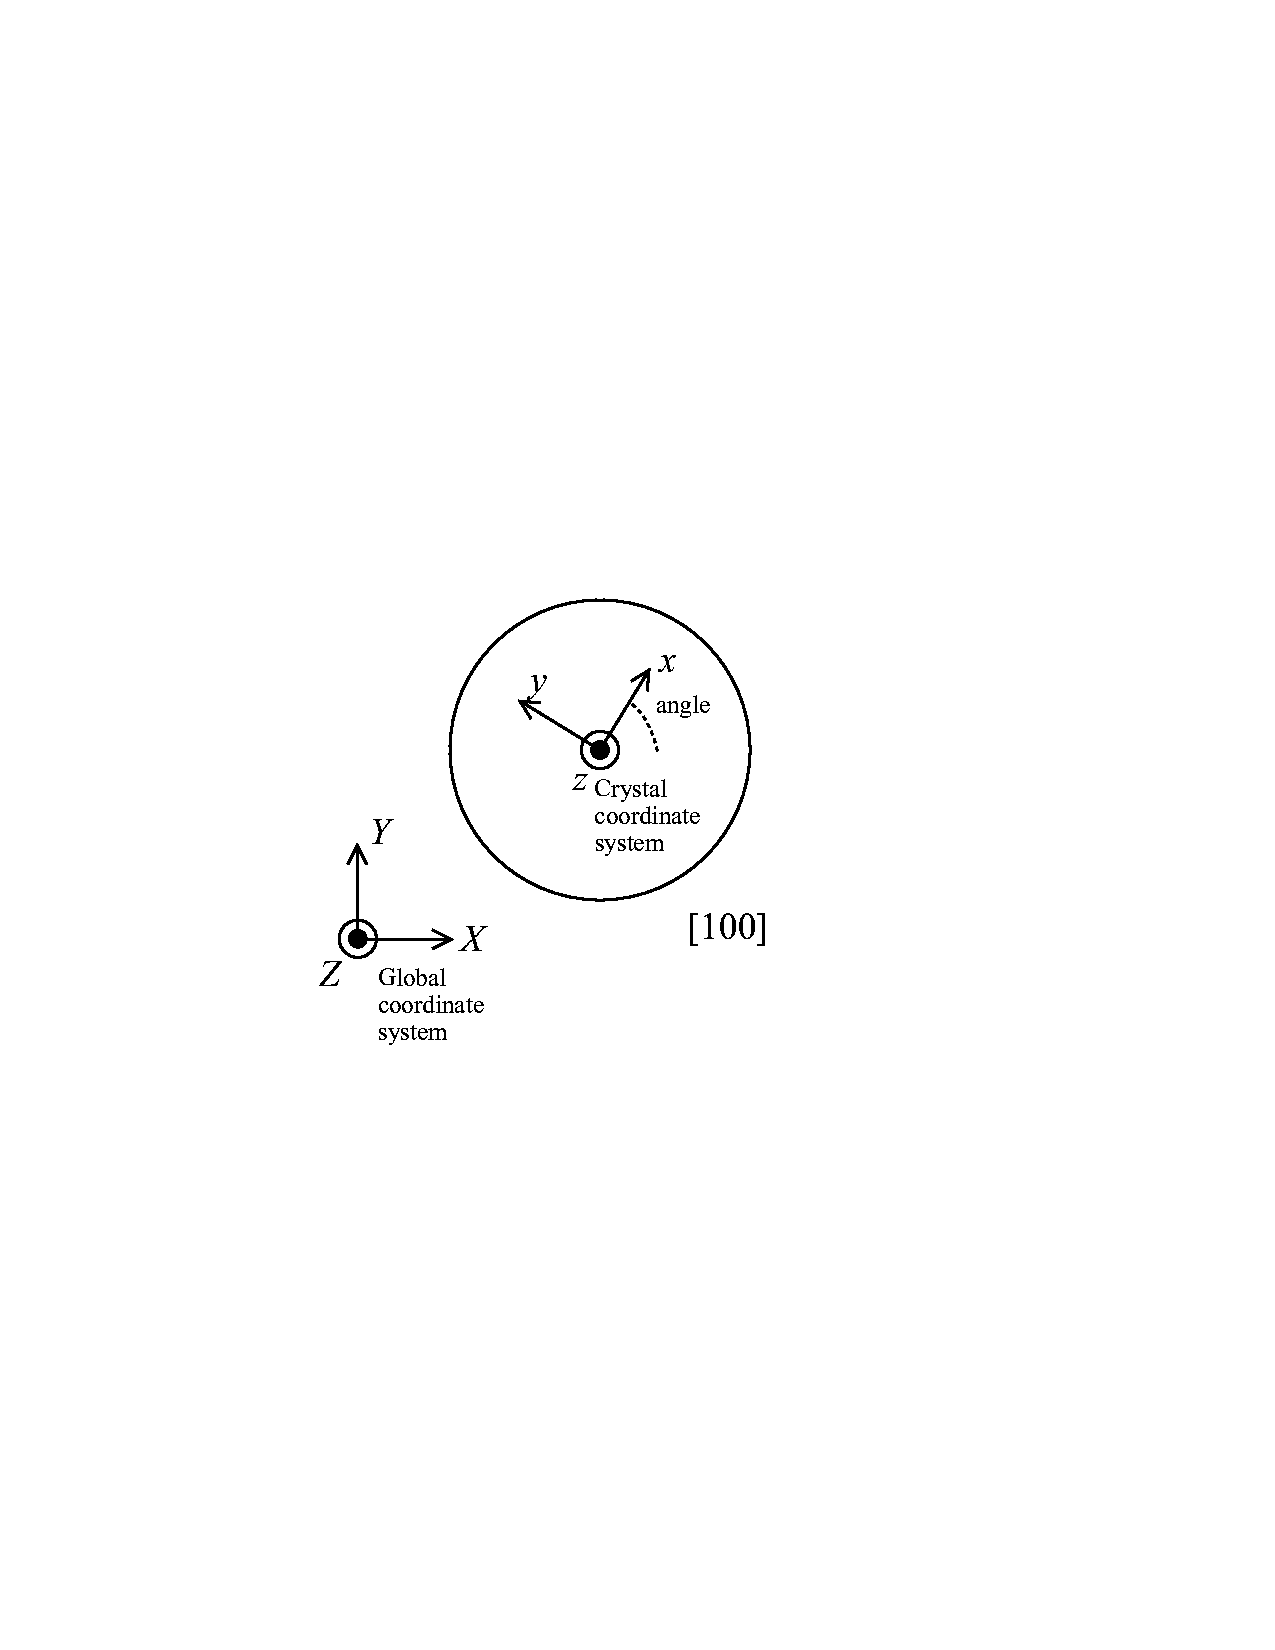
\includegraphics[trim=1.2in 4.0in 3.2in 3.0in, clip, height=2in]{fig/crystalaxis100.pdf}
    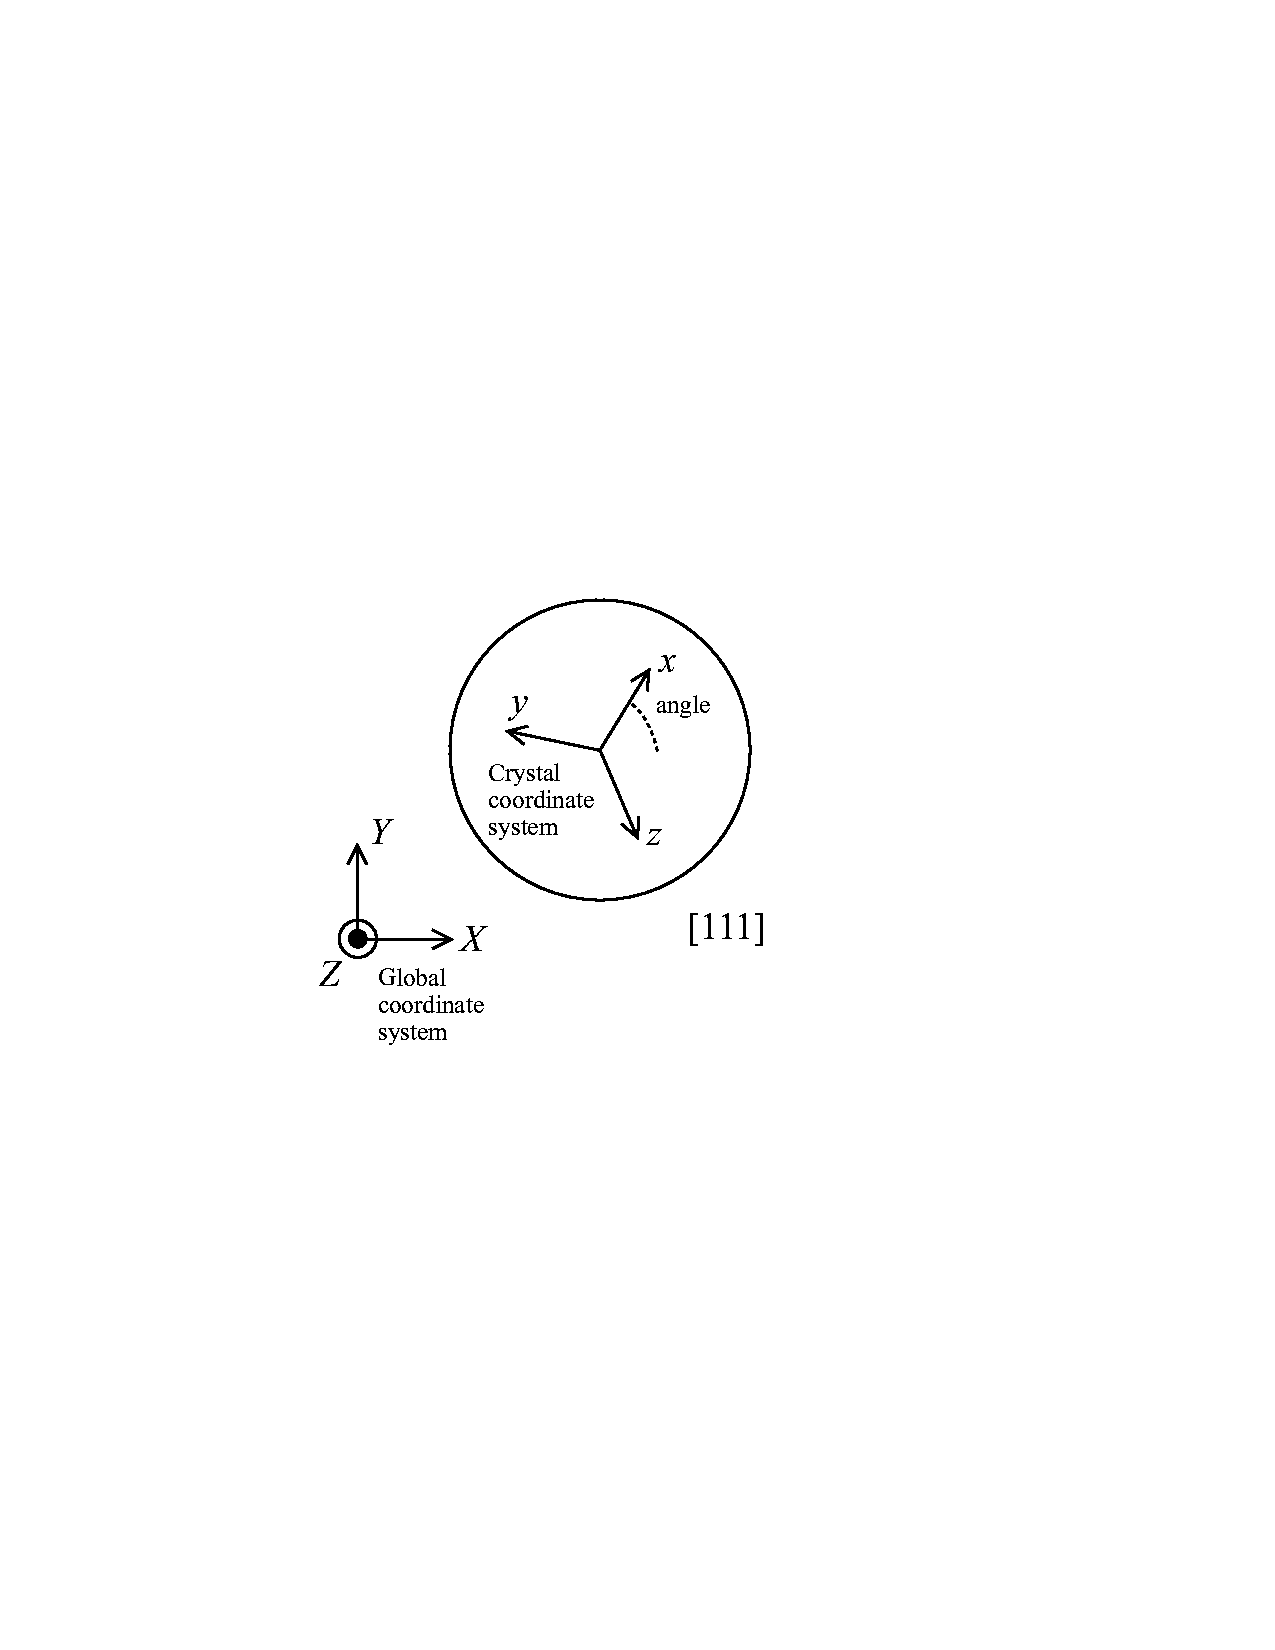
\includegraphics[trim=1.2in 4.0in 3.2in 3.0in, clip, height=2in]{fig/crystalaxis111.pdf}
    \caption{Crystal orientation (wafer and angle)}
    \label{fig:CrystalOrientation}
    \end{figure}
\end{codelist}

\begin{verbatim}
function isotropic_elasticity(mtype, etype, D)
function cubic_elasticity(mtype, etype, axis1, axis2, D)
function hexagonal_elasticity(mtype, etype, axis1, axis2, D)
\end{verbatim}
\begin{verbatim}
function isotropic_thermoelasticity(mtype, etype, Db)
function cubic_thermoelasticity(mtype, etype, axis1, axis2, Db)
\end{verbatim}
\begin{verbatim}
function piezoelectric_elasticity(mtype, etype, axis1, axis2, Db)
\end{verbatim}
